\documentclass[hidelinks,a4paper,12pt, nofootinbib]{article}
\usepackage[width=15.5cm, left=3cm, top=2.5cm, right=2cm, left=2cm, height= 24.5cm]{geometry}
\usepackage[spanish]{babel}
\usepackage[utf8]{inputenc}
\usepackage[T1]{fontenc}
\usepackage{xspace}
\usepackage{xargs}
\usepackage{fancyhdr}
\usepackage{lastpage}
\usepackage{caratulaMetNum}
\usepackage[bottom]{footmisc}
\usepackage{amssymb}
\usepackage{algorithm}
\usepackage[noend]{algpseudocode}

\usepackage{graphicx}
\usepackage{sidecap}
\usepackage{amsmath}
\usepackage{wrapfig}
\usepackage{caption}

\usepackage{hyperref}
\hypersetup{
  colorlinks   = true, %Colours links instead of ugly boxes
  urlcolor     = blue, %Colour for external hyperlinks
  linkcolor    = blue, %Colour of internal links
  citecolor   = red %Colour of citations
}

\usepackage{comment}

\usepackage[
  backend=bibtex,
  style=alphabetic
]{biblatex}
\addbibresource{bibliografia.bib}


\captionsetup[table]{labelsep=space}


\setlength{\parindent}{4em}
\setlength{\parskip}{0.5em}


%%fancyhdr
\pagestyle{fancy}
\thispagestyle{fancy}
\addtolength{\headheight}{1pt}
\lhead{Métodos Numéricos: TP2}
\rhead{$2º$ cuatrimestre de 2015}
\cfoot{\thepage\ / \pageref{LastPage}}
\renewcommand{\footrulewidth}{0.4pt}

%%caratula
\materia{Laboratorio de Métodos Numéricos}
\titulo{Trabajo Práctico Número 2}
\subtitulo{\emph{Ohhh solo tiran $\pi$-edras\dots}}
%\grupo{Grupo 12}
\integrante{Ciruelos Rodríguez, Gonzalo}{063/14}{gonzalo.ciruelos@gmail.com}
\integrante{Costa, Manuel José Joaquín}{035/14}{manuc94@hotmail.com}
\integrante{Gatti, Mathias Nicolás}{477/14}{mathigatti@gmail.com}

\abstracto{asdf}

\palabraClave{key1}
\palabraClave{key2}
\palabraClave{key3}
\palabraClave{key4}

\begin{document}
\maketitle

\tableofcontents
\newpage

\section{Introducción teórica}

El objetivo del presente informe es resolver un problema práctico mediante el modelado matemático del mismo. Este problema consiste en considerar la sección horizontal de un horno de acero cilíndrico, y dadas las temperaturas en el interior y en el exterior de este, analizar si se encuentra en peligro o no.

Para ello, se debe encontrar una cierta isoterma, que si se encuentra muy cerca (para algún significado de la palabra muy) de la pared del horno, consideraremos que el sistema se encuentra en peligro.

Para modelar la difusión de la temperatura, utilizaremos la ecuación de Laplace.

\begin{equation}\label{eq:calor}
\frac{\partial^2T(r,\theta)}{\partial r^{2}}+\frac1r \frac{\partial^2 T(r,\theta)}{\partial r} + \frac{1}{r^2} \frac{\partial T(r, \theta)}{\partial \theta^2} = 0.
\end{equation}

Como puede verse en la ecuación (\ref{eq:calor}), esta ecuación depende de variables que son continuas, lo que es matemáticamente válido, pero computacionalmente imposible (a menos que se haga simbólicamente) de calcular.

Para resolver este problema computacionalmente, debemos discretizar el dominio del problema en coordenadas polares. Por eso consideramos una particion $0 < \theta_0 < \theta_1 < ... < \theta_n = 2\pi$ en $n$ ángulos discretos, con $\theta_i - \theta_{i-1} = \Delta\theta$ constante, y una partición $r_i = r_0 < r_1 < ... < r_m = r_e$ en $m+1$ radios discretos con $r_j - r_{j-1} = \Delta r$ para $j = 1,...,m$.

Entonces ahora, aproximando las derivadas numéricamente utilizando idea del cociente incremental con diferencias finitas podemos obtener un sistema de ecuaciones lineales que describe a el sistema. La formulación detallada del sistema se encuentra en el desarrollo. Para una exposición más completa del tema de resolución de ecuaciones diferenciales con derivadas parciales mediante diferencias finitas se puede consultar \cite[Cap. 11]{burden}.

Además, como explicaremos más adelante, la matriz que determina el sistema del problema tiene una forma muy especial, denominada ``banda''. Esto nos permite asegurar propiedades de la matriz, que serán útiles a la hora de implementar los métodos o intentar optimizarlos.

Para resolver estos sistemas, utilizaremos los dos métodos vistos en clase, eliminación Gaussiana y factorización LU. Por otra parte, como explicaremos mejor y también demostramos en el anexo, podemos realizar estos métodos sin utilizar pivoteo, dado que nunca aparecerá ningun $0$ en la diagonal cuando triangulemos la matriz.



\newpage

\section{Desarrollo}
\subsection{Convenciones}

\subsection{Métodos numéricos usados}

Como dijimos en la introducción, nuestro objetivo será, dada una matriz de transición $P$, encontrarle un autovector de autovalor asociado igual a 1 a su transpuesta. (Usamos la transpuesta por comodidad notacional).

\[P^t x = x\].


\subsubsection{Método de la potencia}
El método de la potencia, dada una matriz A, produce un autovalor $\lambda$ y un autovector asociado a $\lambda$, $v$ no nulo. El método es iterativo, y se puede encontrar una mejor explicación sobre él en \cite[Cap. 5.8.1]{dahlquist}. 

Consiste en tomar un $x^{(0)}$ inicial, y luego construir una sucesión $\{x^{(k)}\}$ de la siguiente manera:

\[x^{(i)} = \frac{A x^{(i-1)}}{||A x^{(i-1)}||}\]

Y entonces, bajo ciertas condiciones, si se toma $k$ lo suficientemente grande, $x^{(k)} \to \overline{x}$, tal que $A\overline{x} = \lambda \overline{x}$, $\lambda$ el autovalor de mayor módulo. Por ello establecemos como criterio de parada que la diferencia entre el vector generado en una iteración y su anterior sea lo suficientemente chica.

Como probamos en \ref{subsub:prop1}, el autovalor de máximo módulo en este caso es 1, aunque puede pasar que $\lambda = -1$ también sea un autovalor. Sin embargo, comenzando con $x^{(0)} = (\frac1n,..., \frac1n)$ inicial, nos aseguramos de que las entradas sean siempre positivas, consiguiendo así un autovector asociado a autovalor $\lambda = 1$.

\subsubsection{PageRank}
PageRank más que un m\'etodo de cómputo es un m\'etodo de modelado. Dado un grafo cuyos nodos representan páginas webs y sus aristas representan links entre las páginas web, nos permitirá modelar un navegante aleatorio utilizando una cadena de Markov. 
Los detalles de la construcción de la cadena y la matriz asociada pueden encontrarse en \cite{Brin1998}.

Proveeremos una breve explicación de como se arma la matriz de transición utilizando un vector fila de la matriz $P$. 
$P_i$ es la $i$-esima fila de la matriz, y su entrada $j$-ésima nos dice la probabilidad que habrá de ir de la página web $i$ a la $j$. A priori una buena aproximación sería

\[ P_{ij} = \begin{cases} 
      \frac{1}{n_i} & \text{si hay un link de $i$ a $j$} \\
       0 & \text{si no}
   \end{cases}
\] 

Donde $n_i$ es la cantidad de links salientes de la página $i$.
El primer problema que se evidencia es que, en general, esta matriz no es de transición, porque si una página web no tiene links salientes, la matriz va a tener toda una fila de ceros. Por eso, en este caso, se agrega una fila que vale toda $(\frac1n, ..., \frac1n)$.

Luego, se introduce el concepto de teletransportación. La idea es que, con una cierta probabilidad $1-c$, el navegante aleatorio puede saltar a cualquier página de toda la red sin importar en cual esté actualmente. Todo esto, nuevamente, esta correctamente explicado en \cite{Brin1998} y \cite{Kamvar2003}.

Luego, puede utilizarse el algoritmo descripto anteriormente para encontrar un autovector de autovalor asociado igual a 1.

En este trabajo en particular, utilizaremos una versión mejorada del m\'etodo de la potencia, adaptada para este problema en particular, propuesta por \cite{Kamvar2003}. Este consiste en separar el único paso del método de la potencia en 3 pasos separados, de tal manera de acelerar el cómputo, aprovechándonos de que la matriz de transición (sin agregarle el factor de teletransportación) es esparsa.

De esta manera, se pueden obtener importantes ganancias en lo que respecta a la performance.

\subsubsection{Método GeM}

El método GeM, propuesto en \cite{Govan2008}, tiene como objetivo adaptar el algoritmo de PageRank para ligas deportivas. La idea es simple, al igual que en el algoritmo original de PageRank, la idea es armar una cadena de Markov y modelar un navegante aleatorio.

En este modelo, se representa una temporada (o una fecha, o un periodo de tiempo cualquiera) como un grafo dirigido y pesado, al igual que en el modelo de PageRank. Sin embargo, en este caso, los pesos de la primera matriz no valen 0 o 1, sino que son el valor absoluto de los puntajes de cada partido.

De esta manera, si el equipo $i$ perdió contra el equipo $j$ por $p$ puntos, en la primera matriz $A$, valdra que $A_{ij} = p$. 

Luego, al igual que en PageRank, las filas de esta matriz que valgan 0 (eso significa que el equipo está invicto hasta el momento) serán completadas y además se agregará el factor de teletransportación, haciendo que todas las entradas de la matriz $P$ sean distintas de 0.

Al igual que antes, nuestro objetivo es encontrar un autovector de autovalor 1 para $P^t$, y para ello utilizaremos el método de la potencia común y corriente.

Es importante notar que este m\'etodo es, a diferencia de el anterior, un m\'etodo que nos indica \emph{cómo} modelar, mientras que el m\'etodo propuesto en \cite{Kamvar2003} lo que hace es tomar un modelo conocido e intentar mejorar su velocidad de cómputo.

\subsubsection{Otros m\'etodos}

Además de los m\'etodos mencionados enteriormente, para cada problema (rankeo de páginas web y de ligas deportivas), utilizaremos un m\'etodo alternativo. 

En el caso de las páginas webs será el conocido como IN-DEGREE, que rankea mejor a aquellas páginas que son mas linkeadas y peor a las que son menos linkeadas. En la parte de experimentación se comparará estos m\'etodos con la requerida profundidad.

En el caso de los rankings de ligas deportivas, utilizaremos el m\'etodo standard de rankeo de cada deporte. En el caso del fútbol, este consiste en caso de empate un punto a cada equipo, y en otro caso darle 3 puntos al equipo ganador y 0 al perdedor.


\subsection{Estructuración del código}
Para el modelado del problema diseñamos tres módulos: Matriz, MatrizDep y Problema. 


\subsubsection{Matriz}
El módulo Matriz es el que se usará para representar a las matrices de conectividad de redes de páginas web.
\paragraph{Representación interna}

Como la matriz de conectividad es en general esparsa (dado que cada página web se conecta en proporción con muy pocas páginas), es conveniente utilizar una representación que aproveche esto. Para eso, vamos a usar una representación conocida como Compressed Row Storage (CRS). Para más información sobre este formato puede consultarse \cite{CRS}.

Elegimos este formato porque será especialmente cómodo a la hora de hacer el producto iterativo del método de la potencia, dado que si queremos hacer $P^tx$, es conveniente poder acceder a $P^t$ por filas fácilmente. 

Además, nos guardamos la cantidad de links que entran y salen de cada nodo. El primer dato será util para calcular la métrica IN-DEGREE, y el segundo dato será util para saber cuánto valdra $P^t_{ij}$, dado que es $\frac{1}{n_j}$, donde $n_j$ es la cantidad de nodos salientes del nodo $j$.

\paragraph{Interfaz}
La interfaz de Matriz provee las siguientes operaciones:\footnote{Cuando se escribe la aridad de la función la misma puede no coincidir con la notación usada en C++. Esto está bien pues lo único que se busca aquí es dar una orientación de lo que hace cada función y no código preciso.}

\begin{itemize}
    \item Matriz(\textbf{ifstream\&} in): constructor de la matriz. Recibe un archivo abierto del cual parseará todos los datos que necesita, en el formato adecuado (SNAP).

    \item \textbf{vector<double>} multiplicar(\textbf{vector<double>} x): El propósito de esta función es autoexplicativo. Devuelve el resultado del producto $Ax$, donde $A$ es la matriz de la clase. El algoritmo que utilizamos es el standard para multiplicar por matrices representadas en CRS, y además, como dijimos anteriormente, dividimos cada entrada por la cantidad de nodos salientes del nodo que corresponda.
\end{itemize}

\subsubsection{MatrizDep}
El módulo MatrizDep es el que se usará para representar a las matrices de conectividad de ligas deportivas.

\paragraph{Representación interna}

Como la matriz de conectividad en este caso, a diferencia del anterior, no suele ser esparsa (de hecho, en el caso general podría aproximarse bastante al grafo completo), entonces no fue necesario utilizar ninguna estructura compleja, y utilizamos simplemente la clásica representación de vector de vectores.

Además fue necesario utilizar otra estructura para almacenar los puntajes de acuerdo a otros métodos de rankeo (por ejemplo, el standard) de la liga deportiva correspondiente.

\paragraph{Interfaz}

La interfaz de MatrizDep provee las siguientes operaciones:
\begin{itemize}
    \item MatrizDep(\textbf{ifstream\&} in): constructor de la matriz. Recibe un archivo abierto del cual parseará todos los datos que necesita, en el formato adecuado (el explicitado en el tp).

    \item \textbf{vector<double>} multiplicar(\textbf{vector<double>} x): autoexplicativa. Devuelve el resultado del producto $Ax$, donde $A$ es la matriz de la clase. El algoritmo que utilizamos es el común y corriente, el mismo que se utiliza al hacer cuentas a mano con matrices.
\end{itemize}




\subsubsection{Problema}
Problema es un módulo que engloba todo lo relacionado al modelado y a la resolución de cada caso particular.


Adicionalmente, tenemos algunas funciones auxiliares: 

\paragraph{Interfaz}

La interfaz de Problema provee funciones utilizadas tanto para el modelado de rankings de páginas web como para el modelado de rankings en ligas deportivas.

Las siguientes operaciones en lo que concierne a la resolución de problemas relacionados con el modelado de páginas web:\footnote{Cuando se escribe la aridad de la función la misma puede no coincidir con la notación usada en C++. Esto está bien pues lo único que se busca aquí es dar una orientación de lo que hace cada función y no código preciso.}

\begin{itemize}
    \item  \textbf{vector<double>} pagerank(\textbf{Matriz} p\_trans, \textbf{double} c, \textbf{double} tolerancia) :
        Se ocupa de aplicar el algoritmo de PageRank sobre la matriz \texttt{p\_trans}, utilizando el algoritmo descripto por \cite[Algoritmo 1]{Kamvar2003}. Además, se testea luego de cada iteración si la diferencia (en norma 1\footnote{$||x||_1 = \sum_i |x_i|$}) es menor que la tolerancia. En ese caso, se termina de iterar y se considera que el vector resultante de la iteración actual es el resultado. 
          
    \item \textbf{vector<uint>} indeg(\textbf{Matriz} p\_trans):  Devuelve el resultado de aplicarle el m\'etodo de rankeo indegree a la red del problema.

A continuación siguen los m\'etodos utilizados para el modelado de rankings de ligas deportivas

  \item \textbf{vector<double>} metodopot(\textbf{MatrizDep} p, \textbf{double} tolerancia):
      M\'etodo de la potencia \emph{vanilla}. Es el que se utilizará para resolver el problema de las ligas deportivas. Obtiene una sucesión de vectores, y cuando su diferencia de norma 1 es menor que la tolerancia pasada como parámetro se termina de iterar.   

\end{itemize}

\subsection{Experimentación}


\newpage

\section{Resultados y discusión}
\subsection{PageRank y páginas web}
Ahora procederemos a analizar, experimentar y discutir los métodos que conciernen al rankeo de páginas Web. Recordemos que en este trabajo se utilizó el modelo PageRank para modelar el rankeo de páginas web utilizando cadenas de Markov y se implementó una versión optimizada especialmente para este problema, presentada en \cite{Kamvar2003}

\subsubsection{Convergencia de PageRank}
Para los experimentos de velocidad de convergencia y rendimiento en general de PageRank utilizamos los datasets de \cite{SNAP}. Para eso, elegimos tres datasets de diferentes tamaños y coeficiente de conectividad \footnote{Con esto nos referimos a que tan conectado está el grafo, esto puede medirse por ejemplo como $\frac{2e}{v(v-1)}$, donde $e$ son las aristas del grafo y $v$ los vertices, dado que el grafo completo tiene $\frac{v(v-1)}{2}$ aristas.}, web-Stanford, web-NotreDame y web-Google.

\begin{figure}[H]
\centering
\begin{tabular}{| c | c | c |}
  \hline
  Dataset & Vértices & Aristas \\ \hline \hline
  web-Stanford & 281.903 & 2.312.497 \\ \hline
  web-NotreDame & 325.729 & 1.497.134 \\ \hline
  web-Google & 916.428 & 5.105.039 \\ \hline
\end{tabular}
\end{figure}


Lo primero que se puede decir de este Datasets es que la diferencia de cantidad de vértices de cada uno nos va a permitir analizar como varía según el tamaño de la red. 

Además, notemos como el dataset web-Stanford está mucho más conectado que el dataset web-NotreDame, dado que tiene menos vértices pero más aristas. Creemos que esto va a impactar negativamente en la performance, dado que sobre una red poco conectada el algoritmo va a converger más rápido.

Eso se puede notar fácilmente si se piensa en el grafo que es totalmente disconexo. En ese caso, todas las entradas de la matriz van a valer $\frac1n$, y el método de la potencia va a converger en un paso.

Otra cosa que podemos pronosticar (en parte porque en \cite{Kamvar2003} pasa eso) es que entre más cercano sea $c$ a 1 (es decir, el navegante aleatorio se teletransporta menos), más lento va a converger.

Al igual que antes, para entender intuitivamente que está pasando, podemos analizar el caso extremo $c = 0$. En este caso, la probabilidad de que el navegante se teletransporte es siempre 1, por lo que volvemos al caso anterior en el que todos los coeficientes de la matriz van a valer $\frac1n$, por lo que se convergerá en un paso.

Concluidas las hipótesis relacionadas a la convergencia del método, procedamos a ver los resultados de los experimentos.


\begin{figure}[H]
\centering
\begin{minipage}{0.48\textwidth}
  \centering
    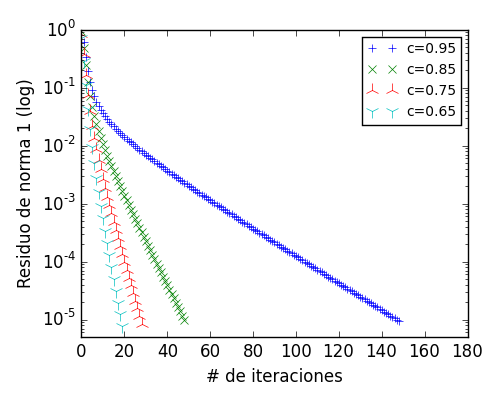
\includegraphics[width=1\textwidth]{imgs/convergencia-stanford.png}
  \caption{\footnotesize{Comparación de la velocidad de convergencia del el método para el dataset web-Stanford.}}
  \label{fig:conv1}
\end{minipage}
\hspace{0.02\textwidth}
\begin{minipage}{0.48\textwidth}
  \centering
    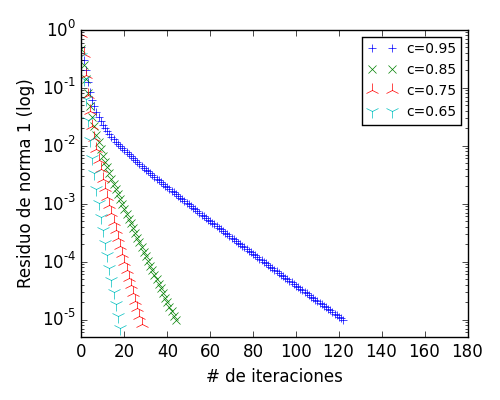
\includegraphics[width=1\textwidth]{imgs/convergencia-notredame.png}
  \caption{\footnotesize{Comparación de la velocidad de convergencia del el método para el dataset web-NotreDame.}}
  \label{fig:conv2}
\end{minipage}
\begin{minipage}{0.5\textwidth}
  \centering
    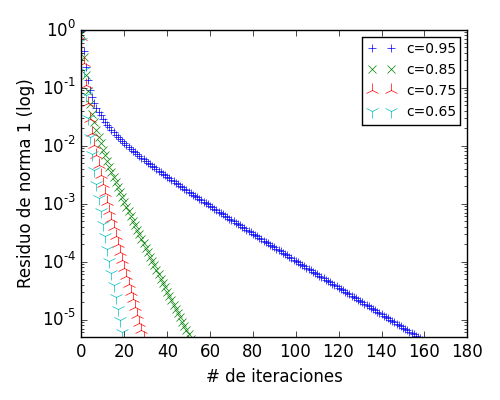
\includegraphics[width=1\textwidth]{imgs/convergencia-google.png}
  \caption{\footnotesize{Comparación de la velocidad de convergencia del el método para el dataset web-Google.}}
  \label{fig:conv3}
\end{minipage}
\end{figure}


Primero notemos algo más o menos sorprendente: la cantidad de iteraciones requeridas por el método no varía demasiado, sobre todo para valores chicos de $c$. Creemos que esto se debe a propiedades generales del método de la potencia, que sin embargo son díficiles de analizar y están fuera del alcance de este trabajo.

Se puede notar además que para los valores más pequeños de $c$ la cantidad de iteraciones correspondientes a cada dataset es prácticamente igual.

Una cosa importante para decir, de la cual vamos a hablar en profundidad más adelante, es que aunque la cantidad de iteraciones sea parecida, el costo de cada iteración es mayor a más grande es la matriz y a más valores no nulos tiene, por lo que las figuras \ref{fig:conv1}, \ref{fig:conv2} y \ref{fig:conv3} no deben intepretarse como el tiempo que requiere el algoritmo para correr.

Sin embargo, una cosa interesante a analizar es qué $c$ usar. Como vimos, usar un $c$ pequeño disminuye el tiempo de cómputo requerido. Sin embargo, disminuir el $c$ también puede impactar en el resultado. Dado que el factor de teletransportación $1-c$ es más alto, de alguna manera el resultado es menos significativo, debido a que se hace más uniforme, como explicamos antes. 
En \cite{Chakrabarti}, por ejemplo, se sugiere que $c$ debería ser elegido basado en la conectividad del grafo.


Otro experimento muy interesante que realizamos es cambiar el criterio de parada del algoritmo iterativo. En particular, lo que hicimos fue cambiar la norma con la que medimos la diferencia entre dos vectores de sucesivas iteraciones. Para ello utilizamos las normas $||-||_1$, $||-||_2$ y $||-||_{\infty}$.

\begin{figure}[H]
\centering

    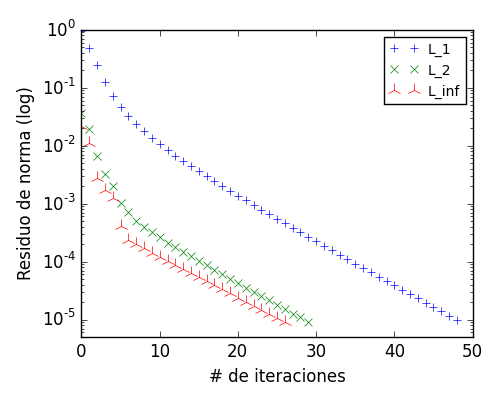
\includegraphics[width=0.6\textwidth]{imgs/convergencia-norma.png}
  \caption{\footnotesize{Comparación de la velocidad de convergencia del el método para el dataset web-Stanford, variando la norma del criterio de parada.}}
  \label{fig:conv-norma}
\end{figure}

Como se observa en la figura \ref{fig:conv-norma}, cuando se utiliza la norma 1 para el criterio de parada, se requieren más iteraciones para terminar. Esto se debe a que la norma 1 es la más \emph{exigente}. 

Se puede probar fácilmente que para todo vector $x$, $||x||_1 \geq ||x||_2 \geq ||x||_{\infty}$ y esto explica claramente los resultados del experimento.



\subsubsection{Rendimiento de PageRank}
A continuación analizaremos el rendimiento del algoritmo de PageRank implementado en este trabajo, es decir, el de \cite{Kamvar2003}. Para ello, utilizaremos los mismos datasets que en la sección anterior.

\begin{figure}[H]
\centering
\begin{tabular}{| c | c | c | c |}
  \hline
  Dataset & Vértices & Aristas & Tiempo (segundos) \\ \hline \hline
  web-Stanford & 281.903 & 2.312.497 & 7.81882 \\ \hline
  web-NotreDame & 325.729 & 1.497.134 & 3.38163 \\ \hline
  web-Google & 916.428 & 5.105.039 & 23.7367 \\ \hline
\end{tabular}

  \caption{\footnotesize{Comparación de los tiempos que requiere el algoritmo para distintos datasets. Fue ejecutado con $c = 0.85$ y $tolerancia = 0.00001$.  Se tomó el promedio de 20 mediciones.}}
  \label{fig:tiempos1}
\end{figure}

Podríamos empezar a sacar conclusiones apresuradas sobre estos datos, pero para que sean más significativos, preferimos realizar otro experimento antes de comenzar el análisis.
Este experimento consiste en dividir el algoritmo en 2: primero el armado de la matriz (recordemos que como representamos la matriz en CRS este no es un paso trivial) y luego el paso de método de la potencia optimizado presentado en \cite{Kamvar2003}.

Esto nos permitirá ver mejor el problema y tener datos más detallados, con el objetivo de poder analizar mejor que es lo que sucede.

\begin{figure}[H]
\centering
\begin{tabular}{| c | c | c | c |}
  \hline
  Dataset & Tiempo total & Armado de matriz & Método de la potencia \\ \hline \hline
  web-Stanford & 7.81882 & 1.8968 & 5.91098 \\ \hline
  web-NotreDame &  3.38163 & 0.978923 & 2.42743 \\ \hline
  web-Google & 23.7367 & 4.30584 & 18.9483 \\ \hline
\end{tabular}

  \caption{\footnotesize{Comparación de los tiempos que requiere el algoritmo para distintos datasets. Fue ejecutado con $c = 0.85$ y $tolerancia = 0.00001$. Se tomó el promedio de 20 mediciones. Todos los tiempos son en segundos. Las sumas probablemente no den bien porque fueron tomadas en diferentes mediciones. }}
  \label{fig:tiempos2}
\end{figure}


Ahora, teniendo toda la información que nos proveen la figura \ref{fig:tiempos1}, \ref{fig:tiempos2} y los experimentos de la sección anterior, podemos hacer un análisis completo y riguroso.

Podemos concluir primero que el paso más costoso del algoritmo es el método de la potencia. Justamente por eso \cite{Kamvar2003} se ocupa de intentar optimizar ese paso, dado que optimizarlo va a impactar fuertemente en el rendimiento general de la aplicación.


Otro aspecto interesante para ver es, como aunque las iteraciones requeridas para cada dataset son bastante similares, el costo de cada operación es muy distinto, pues el tamaño de los vectores varía, y las entradas no nulas de la matriz son distintas. 

De hecho, este experimento nos permite confirmar que el paso más costoso es realizar el producto de la matriz y el vector $P^t x^{(k)}$, ya que se puede ver como el método de la potencia en el caso de web-NotreDame tarda menos que en el caso de web-Stanford, aunque los vectores sean más largos. 

Esto se debe a que la matriz de web-NotreDame es más esparsa, y al multiplicar $Ax$ con $A$ representada en CRS, el costo resulta lineal en la cantidad de elementos no nulos de la matriz. Esta última está intimamente relacionada con la cantidad de aristas del grafo. De esta manera se explica fácilmente el comportamiento a priori extraño de el algoritmo sobre estos datasets.



\newpage
\subsection{PageRank y ligas deportivas}
%\input{asdf.tex}
\newpage

\section{Conclusiones}
A continuación pasamos en limpio las conclusiones a las que llegamos con la realización del presente trabajo práctico.

Con respecto al método pagerank:
\begin{itemize}
	\item En lo concerniente a la convergerncia del método concluimos que:
		\begin{itemize}
			\item Para un mismo valor de $c$, la cantidad de iteraciones requeridas para distintos datasets varía poco, especialmente si $c$ es chico. Si $c$ es muy cercano a 1, entonces la cantidad de iteraciones es menor para grafos más disconexos.
			\item Entre más chico sea el valor de $c$, más rápido va a converger pagerank. Sin embargo, esto también produce que el resultado sea menos significativo, por lo cual es importante tener un buen criterio para la elección del $c$, por ejemplo, considerando la conectividaad del grafo.
			\item Al modificar la norma que usamos para determinar el criterio de parada, vemos que usar una norma $p$ disminuye la cantidad de iteraciones cuanto mayor es $p$, pero al mismo tiempo genera que el resultado sea menos preciso. De forma similar, un $p$ más chico produce el efecto contrario.
		\end{itemize}
	\item Sobre la performance del método, vimos que el paso más costoso del algoritmo es realizar el método de la potencia. Pese a que la cantidad de iteraciones para dos datasets distintos fuera prácticamente igual, el tiempo de cómputo efectivo era distinto pues el costo de realizar cada producto de matriz por vector dependía linealmente de la cantidad de coeficientes no nulos de la matriz (debido a la representación CRS utilizada para la misma). Por lo tanto, para matrices más esparsas (correspondientes a grafos más disconexos), se requiere menos tiempo de cómputo.
	\item En lo respectivo al análisis cualitativo, concluimos que pagerank permite conseguir rankings más realistas que In-Deg, como resultado de considerar no solo la cantidad de enlaces entrantes sino también la importancia relativa de los mismos. Además, vimos que pagerank le permite a cada página mejorar parcialmente su posición al agregar un mayor número de enlaces salientes. Como trabajo a futuro se plantea el generalizar y profundizar las propiedades vistas. 
\end{itemize}

Con respecto al modelo GeM:
\begin{itemize}
	\item Vimos que el método propuesto por Govan et al. no es \emph{democrático}, en el sentido de que tiene mucha más relevancia sacarle un diferencia positiva a un equipo que está bien rankeado que a uno que no lo está. Esta es una clara diferencia  con el método tradicional de rankeo del fútbol, en la cual ganarle a cualquier equipo da la misma cantidad de puntos. Así mismo, las diferencias grandes de marcador son un factor clave pues favorecen más al vencedor, cosa que no se da con el método clásico.
	\item En la misma línea de lo anterior, vimos que el valor de $c$ afecta de forma directa la calidad del rankeo: si bien en términos generales puede no producir grandes cambios, el tomar un valor muy cercano a 1 genera que equipos de un bajo rendimiento general puedan aprovecharse demasiado de una victoria aislada a algún equipo bien posicionado. Mientras tanto, tomar un valor más cercano a 0 amortigua este efecto, dándole mayor importancia a la cantidad de partidos ganados. Particularmente, llegamos a la conclusión de que un valor para $c$ cercano a $0.35$ genera rankings sensatos (al menos para el caso de una liga de las características mencionadas en la sección (\ref{subsec:ligas})), logrando entonces un buen promedio entre la importancia de vencer a equipos importantes, así como marcar diferencias amplias de goles, y tener un \emph{ratio} razonablemente bueno de victorias/derrotas. Esto es especialmente importante en el caso del fútbol donde, a diferencia de otros deportes como el rugby o el tennis, no es raro que se produzcan resultados sorpresivos.  
	\item Por otro lado, encontramos que el no considerar los empates con el método GeM puede traer disparidades. Sin embargo, un análisis más profundo sobre este aspecto queda pendiente para trabajos posteriores, así como la realización de variaciones del método que manejen el caso de los empates de forma distinta. Algunas ideas en este sentido podrían ser poner en la posición $(i,j)$ y $(j,i)$ de la matriz de adyacencias la cantidad de goles por la que empataron los equipos $i$ y $j$, o bien, siempre poner 1. También queda en el tintero probar la versión generalizada del modelo GeM que se propone al final de \cite{Govan2008}, con la cual se podrían considerar otras estadísticas como posesión del balón, cantidad de tarjetas, etc.
\end{itemize}
\newpage

\section{Apéndices}
\subsection{Proposiciones}

\subsubsection{Proposición 1}
\label{subsub:prop1}
Si $P \in R^{n\times n}$ es una matriz de transición, es decir $0 \leq P_{ij} \leq 1$, y $\sum_j P_{ij} = 1 \ \forall i\in\{1,...,n\}$, entonces el mayor autovalor en módulo de $P^t$ es 1, y en particular tiene a 1 como autovalor (eventualmente podría tener tamién a -1).

\textbf{Demostración} Primero veamos que si $\lambda$ es autovalor de $P^t$, entonces $|\lambda| \leq 1$.

Vale que $\rho(P^t) \leq ||P^t||$, $\rho(P^t)$ el radio espectral y $||-||$ cualquier norma inducida. En particular, si tomamos la norma 1, $||P^t||_1 = 1$, pues todas las columnas suman 1, pues $P$ es de transición. Entonces $|\lambda| \leq \rho(P^t) \leq 1$.

Ahora, como las filas de $P$ suman 1, si multiplico $P (1, ..., 1)^t = (1, ..., 1)^t$. Es decir que 1 es autovalor de $P$. Entonces, como $P$ y $P^t$ tienen los mismos autovalores, 1 es autovalor de $P^t$, que es lo que queríamos ver.

\textbf{Observación} Probamos que 1 es efectivamente autovalor de la matriz, pero nada nos garantiza que -1 no lo sea. Sin embargo, si al aplicar el método de la potencia empezamos con un vector de todas entradas positivas (como lo hacemos), el resultado final también tendrá todas entradas positivas, resultando en un autovector asociado a autovalor 1.



\newpage
% si se descomenta esto, aparecen todas las cosas de la bibliografia, hasta
% las que nunca fueron citadas en el TP. es una eleccion de diseño.
% \nocite{*}
\printbibliography



\end{document}
